\documentclass[a4paper, 11pt]{article}
\usepackage[spanish]{babel}
\usepackage[utf8]{inputenc}
\usepackage{graphicx}
\usepackage{multirow}

\begin{document}
\pagenumbering{gobble}
\begin{titlepage}
   \begin{center}
   \includegraphics[width=6cm]{recursos/logo_UNC}
   
   \Huge
   \textbf{Propuesta de Práctica Profesional Supervisada}
   
   \vspace{0.5cm}
   \LARGE
   Investigación y aprendizaje sobre herramientas de desarrollo en el kernel de FreeBSD

   \vspace{0.5cm}
   \large
   \underline{\textbf{Alumno:}}
   
   \textbf{Rivero, Franco Fabián \\38111351}
   \vspace{0.2cm}
   
   \underline{\textbf{Tutor:}}
   
   \textbf{Maximiliano Eschoyez}
   
    \vspace{0.2cm}
   
   \underline{\textbf{Supervisor:}}
   
   \textbf{Nicolás Papp}
   \vspace{0.5cm}
   
   \textit{Facultad de Ciencias Exactas, Físicas y Naturales}\\
   \textit{Universidad Nacional de Córdoba}\\
   \textit{Córdoba, 2021}
   
   \vspace{1cm}
   
   
\includegraphics[width=5cm]{recursos/logo}
\end{center}  
\end{titlepage}

\section*{Descripción de actividades}

\vspace{0.4cm}
\large
Se realizará una investigación sobre FreeBSD, cambios dentro de su kernel, desarrollo de nuevos módulos. Basándome en el proyecto final \textbf{Modelado del planificador a corto plazo con redes de Petri} de los ingenieros Nicolás Papp y Tomás Turina se realizará una investigación de las modificaciones hechas. Se dividirá la tarea en algunas etapas para simplificar la complejidad de la tarea.
En una primera etapa se investigará las herramientas a utilizar y lograr preparar el entorno de desarrollo en una máquina virtual. En la segunda parte se buscará automatizar el armado del entorno y buscar herramientas para medir el rendimiento de los distintos planificadores a corto plazo en la plataforma FreeBSD.

\newpage

\section*{Objetivos}
\subsection*{Objetivos generales}

El estudiante aprenderá sobre tecnologías existentes para el desarrollo en kernel de un sistema operativo, más específicamente en FreeBSD. También adquirirá experiencia en investigación, resolución de problemas y herramientas de virtualización con las tecnologías que se están utilizando hoy en día.

\vspace{0.7cm}
\subsection*{Objetivos específicos}

Proyecto: Investigación y aprendizaje sobre herramientas de desarrollo en el kernel de FreeBSD.

\vspace{0.5cm}
El proyecto a llevar a cabo se divide en objetivos específicos:

\begin{enumerate}
	\item Instalación del sistema operativo FreeBSD en una máquina virtual
	\item Instalación de paquetes y configuración del sistema operativo
	\item Compilación de un kernel de FreeBSD
	\item Utilizar herramientas viables para lograr automatizar y facilitar un entorno para poder compilar FreeBSD
	\item Automatizar la creación de máquinas virtuales de prueba
	\item Utilizar herramientas para medir el rendimiento del sistema
	\item Compilar el kernel con los cambios realizados por Nicolas y Tomas.
\end{enumerate}
\newpage
\section*{Cronograma de actividades y distribución de carga horaria}
	
	La finalización de la PPS se prevé en un lapso de 200 hs. de trabajo, con dedicación mixta con la siguiente distribución:
	
	\begin{itemize}
		\item \textbf{Tarea 1 (10 hs):} Investigación sobre el sistema operativo FreeBSD.
		\item \textbf{Tarea 2 (15 hs):} Instalación de FreeBSD en una máquina virtual.
		\item \textbf{Tarea 3 (15 hs):} Configuración de FreeBSD.
		\item \textbf{Tarea 4 (25 hs):} Compilación del kernel dentro de FreeBSD.
		\item \textbf{Tarea 5 (25 hs):} Compilación con un kernel modificado dentro de FreeBSD.
		\item \textbf{Tarea 6 (10 hs):} Investigar sobre herramientas de deployment y automatización
		\item \textbf{Tarea 7 (50 hs):} Automatización de generación de máquinas virtuales
		\item \textbf{Tarea 8 (25 hs):} Análisis de viabilidad de herramientas de profiling 
		\item \textbf{Tarea 9 (25 hs):} Compilación de kernel con el scheduler modificado para soportar redes de Petri
	\end{itemize}

\subsection*{Diagrama de Gantt}
	\vspace{1cm}

	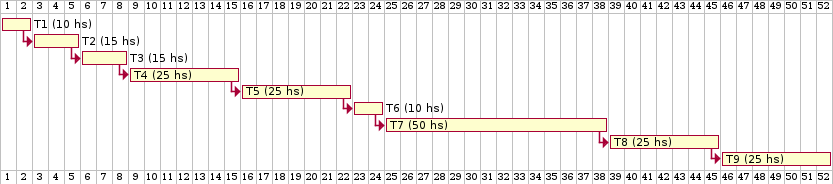
\includegraphics[width=16cm]{recursos/gantt_diagram}


\end{document}